\chapter{Thuật toán Lập lịch trình Không gian, Thực nghiệm Đối sánh và Tích hợp Ứng dụng}
\label{ch:thuc-nghiem}

\section{Thuật toán Lập lịch trình phân cụm không gian}
\label{sec:ch2-planner}

\subsection{Bài toán phân cụm địa lý theo sông Hương}
\label{subsec:ch2-clustering}

Thành phố Huế sở hữu một đặc trưng địa lý tự nhiên chi phối toàn bộ cấu trúc giao thông đô thị: sông Hương chảy qua trung tâm, chia cắt thành phố thành hai bờ Bắc và bờ Nam với số lượng cầu kết nối có hạn. Bờ Bắc là không gian văn hóa di sản cung đình cổ kính tập trung xung quanh Quần thể Kinh thành Huế, Chùa Thiên Mụ và Chợ Đông Ba; trong khi bờ Nam là khu đô thị hiện đại và hành lang phát triển về phía các quần thể lăng tẩm triều Nguyễn (Lăng Tự Đức, Lăng Khải Định) cùng các làng nghề truyền thống như Làng hương Thủy Xuân.

Nếu du khách hoặc các trợ lý ảo lập lịch trình di chuyển xen kẽ tùy tiện giữa hai bờ trong cùng một buổi sáng hoặc buổi chiều, thời gian lãng phí cho việc vượt cầu qua lại và nguy cơ tắc nghẽn giao thông giờ cao điểm sẽ làm giảm sút nghiêm trọng trải nghiệm du lịch. Để giải quyết triệt để vấn đề này, giải thuật Spatial Itinerary Planner phân chia không gian du lịch Huế thành ba cụm địa lý độc lập (Spatial Clusters):

Cụm 1 -- Bờ Bắc (Di sản Kinh thành và Cổ tự): Bao gồm Đại Nội Huế, Kỳ Đài, Bảo tàng Cổ vật Cung đình Huế, Chợ Đông Ba, Hồ Tịnh Tâm và Chùa Thiên Mụ. Toàn bộ các điểm đến trong cụm này nằm gọn trong bán kính 3~km bên bờ Bắc sông Hương.
Cụm 2 -- Bờ Nam (Lăng tẩm vương triều và Làng nghề): Bao gồm Lăng Tự Đức, Lăng Đồng Khánh, Đồi Vọng Cảnh, Làng hương Thủy Xuân và Lăng Khải Định. Các điểm đến này liên kết thuận tiện theo trục đường Huyền Trân Công Chúa và Khải Định.
Cụm 3 -- Ngoại ô và Văn hóa Làng quê: Bao gồm Lăng Minh Mạng, Cầu ngói Thanh Toàn, Đầm Chuồn (phá Tam Giang) và Làng cổ Phước Tích, thích hợp cho các chuyến khám phá bán nhật hoặc nguyên nhật dã ngoại.

Quy trình phân luồng và trải nghiệm thực tế của người dùng được mô tả trực quan trên Hình \ref{fig:user-scenario-flow}.

\begin{figure}[htbp]
\centering
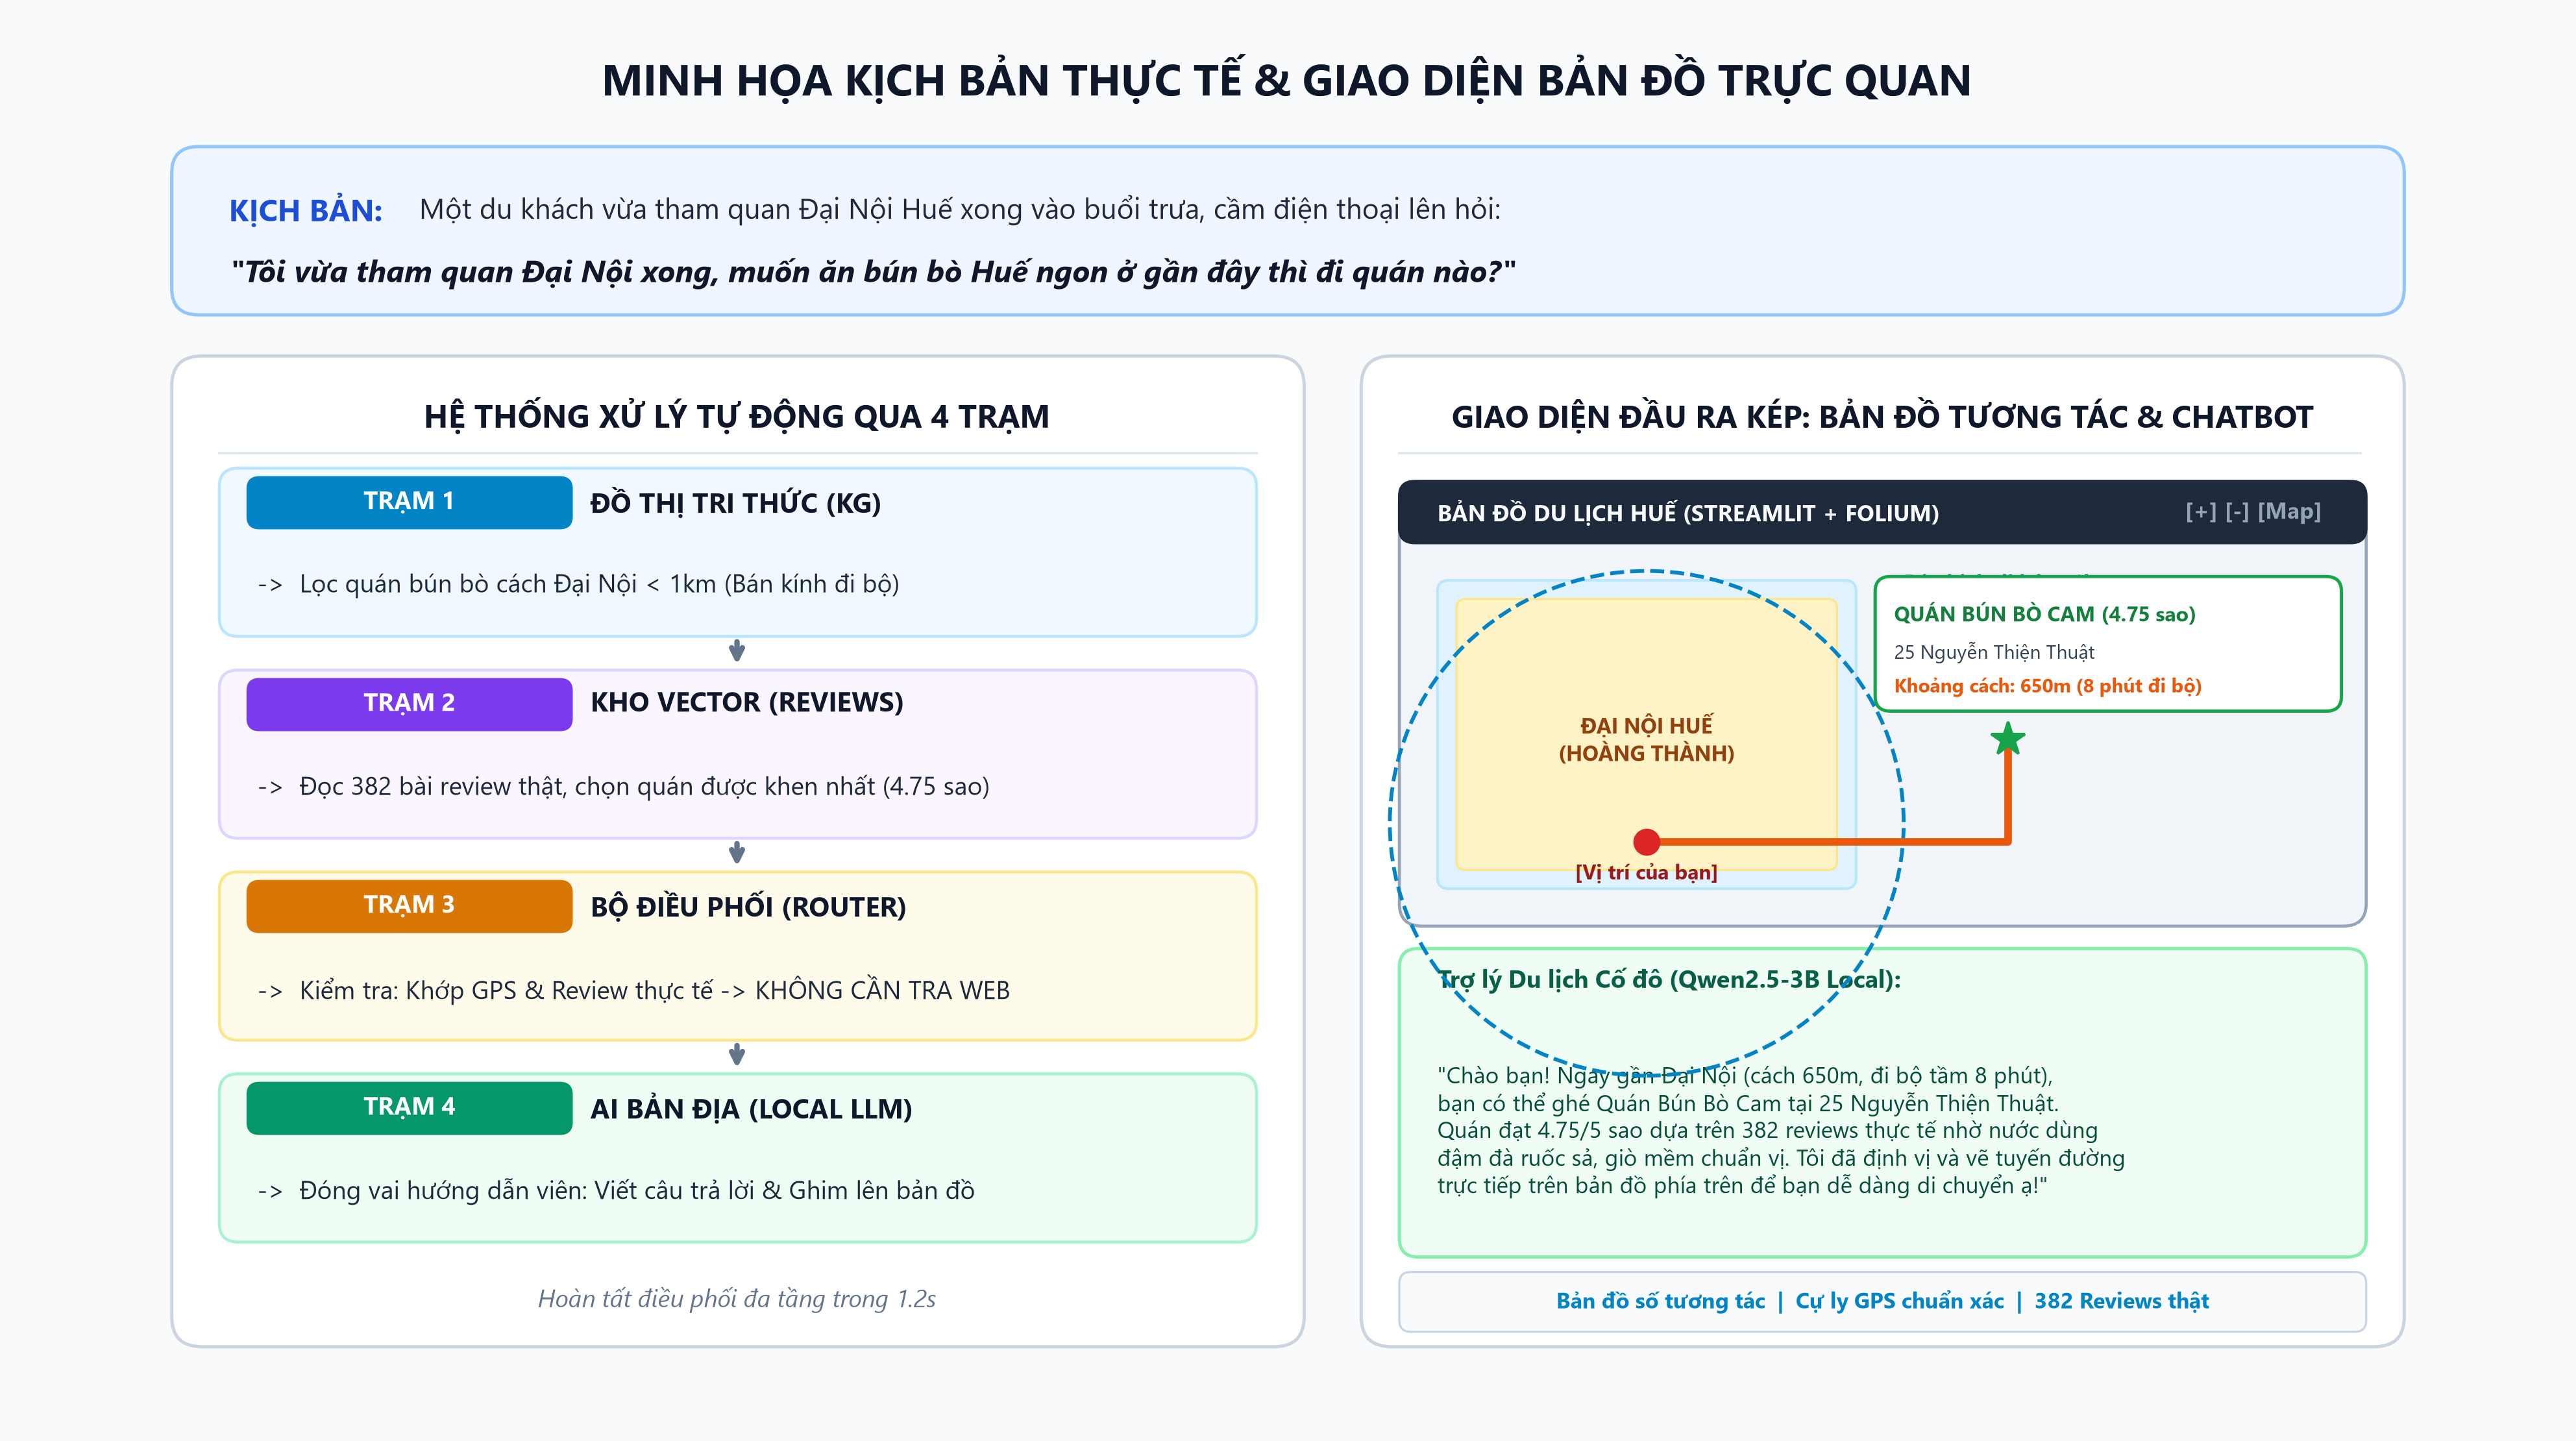
\includegraphics[width=0.92\textwidth]{img/user_scenario_demo_flow.png}
\caption{Kịch bản luồng tương tác và gợi ý lịch trình phân cụm không gian của hệ thống}
\label{fig:user-scenario-flow}
\end{figure}

Từ luồng kịch bản tại Hình \ref{fig:user-scenario-flow}, giải thuật lập lịch trình vận hành theo nguyên tắc tối ưu hóa từng ngày: mỗi ngày du khách chỉ khám phá trọn vẹn một cụm địa lý duy nhất. Tại mỗi điểm tham quan chính (Anchor POI), hệ thống tự động quét đồ thị tri thức để tìm kiếm các cơ sở ẩm thực lân cận trong bán kính $d \le 1,5\text{ km}$ phục vụ đúng món đặc sản theo sở thích của du khách, bảo đảm hành trình di chuyển liền mạch và hoàn toàn không bị nhảy bờ sông Hương ziczac.

\subsection{Giải thuật tối ưu hóa lịch trình đa ngày}
\label{subsec:ch2-algorithm}

Thuật toán lập lịch trình nhận đầu vào gồm số ngày lưu trú $K \in \{1, 2, 3\}$, danh sách các sở thích cá nhân (ẩm thực, di tích lịch sử, cảnh quan thiên nhiên), và địa điểm xuất phát (khách sạn lưu trú). Giải thuật trải qua ba bước xử lý chính:

Bước 1: Lựa chọn cụm không gian tối ưu cho từng ngày tham quan. Với lịch trình 1 ngày, hệ thống ưu tiên Cụm 1 (Bờ Bắc) cho buổi sáng và Cụm 2 (Bờ Nam) cho buổi chiều để bảo đảm trải nghiệm các di sản cốt lõi nhất. Với lịch trình 2 ngày hoặc 3 ngày, mỗi cụm được phân bổ trọn vẹn cho một ngày riêng biệt.

Bước 2: Sắp xếp thứ tự tham quan bên trong cụm (Intra-cluster Routing). Dựa trên ma trận khoảng cách Haversine giữa các điểm đến trong cụm, giải thuật áp dụng phương pháp tham lam kết hợp tìm kiếm cục bộ (Greedy Nearest Neighbor with 2-Opt refinement) để tìm chu trình di chuyển có tổng khoảng cách ngắn nhất:
\begin{equation}
    \min_{\pi} \sum_{i=1}^{m-1} d(v_{\pi(i)}, v_{\pi(i+1)})
    \label{eq:routing-opt}
\end{equation}
trong đó $\pi = (\pi(1), \pi(2), \dots, \pi(m))$ là hoán vị thứ tự ghé thăm $m$ điểm tham quan trong ngày, và $d(\cdot, \cdot)$ là khoảng cách Haversine tính theo công thức (\ref{eq:haversine}).

Bước 3: Ghép nối ẩm thực thông minh (Culinary Ingestion). Tại điểm dừng chân buổi trưa (thường là điểm di tích thứ hai trong buổi sáng) và điểm kết thúc buổi chiều, giải thuật truy vấn cạnh $\text{NEAR\_BY}$ kết hợp cạnh $\text{SERVES}$ để chọn ra nhà hàng có điểm tin cậy $\text{Conf}(u, m) \ge 0,70$ và khoảng cách $d \le 1,5\text{ km}$ gần nhất.

\section{Thiết lập thực nghiệm và Bộ dữ liệu kiểm thử chuẩn}
\label{sec:ch2-setup}

\subsection{Môi trường phần cứng và khung phần mềm}
\label{subsec:ch2-environment}

Toàn bộ các thí nghiệm kiểm chứng định lượng được triển khai trên môi trường máy trạm cá nhân nhằm chứng minh tính khả thi thực tế của giải pháp: bộ xử lý trung tâm Intel Core i5 / AMD Ryzen 5, bộ nhớ trong 16GB RAM, bộ xử lý đồ họa NVIDIA GeForce RTX 3050 Laptop với 4GB VRAM, hệ điều hành Windows 11, môi trường phát triển Python 3.12, và máy chủ suy luận cục bộ Ollama phiên bản 0.4.

Mô hình ngôn ngữ lớn được sử dụng là Qwen2.5-3B-Instruct (phiên bản định lượng Q4\_K\_M, chiếm dụng khoảng 2,2GB VRAM), bảo đảm thời gian tải mô hình tức thì và năng lực sinh văn bản tiếng Việt tốc độ cao (trên 35 tokens/giây) mà hoàn toàn không phụ thuộc vào kết nối mạng Internet hay chi phí gọi API đám mây.

\subsection{Bộ kiểm thử Benchmark 12 kịch bản du lịch Huế}
\label{subsec:ch2-benchmark-suite}

Để đánh giá toàn diện năng lực của hệ thống, nghiên cứu xây dựng một bộ dữ liệu kiểm thử chuẩn (Benchmark Test Suite) bao gồm 12 kịch bản đại diện thực tế, bao quát ba nhóm bài toán du lịch phổ biến nhất:

Nhóm 1 -- Không gian kết hợp Ẩm thực (Spatial + Culinary Query): Gồm 4 câu hỏi kiểm tra khả năng tìm kiếm quán ăn phục vụ đúng món đặc sản lân cận một điểm di tích (ví dụ: tìm quán bún bò chuẩn vị gần Đại Nội, quán bánh bèo gần lăng Tự Đức, quán cơm hến gần cồn Hến).
Nhóm 2 -- Khám phá lân cận (Spatial Proximity Exploration): Gồm 4 câu hỏi kiểm tra khả năng đề xuất các điểm danh thắng lân cận trong bán kính đi bộ quanh một điểm mốc (ví dụ: các điểm tham quan gần Chùa Thiên Mụ, các điểm ngắm hoàng hôn gần Đồi Vọng Cảnh).
Nhóm 3 -- Lập lịch trình tổng hợp (Itinerary Planning): Gồm 4 câu hỏi yêu cầu thiết kế lịch trình 1 ngày, 2 ngày và 3 ngày tại Huế có tích hợp đầy đủ di tích, ẩm thực và phương án di chuyển.

\section{Kết quả thực nghiệm đối sánh định lượng}
\label{sec:ch2-results}

\subsection{Hệ thống các mô hình đối chuẩn và Tiêu chí đo lường}
\label{subsec:ch2-metrics}

Nghiên cứu tiến hành đo lường và đối sánh định lượng giữa ba phương pháp phương pháp luận đại diện:
Mô hình M1: Zero-shot LLM (Sử dụng trực tiếp mô hình Qwen2.5-3B-Instruct không có cơ chế RAG).
Mô hình M2: Naive RAG (Cơ chế RAG vector truyền thống sử dụng ChromaDB với độ đo Cosine Similarity).
Mô hình M3: Spatial GraphRAG (Phương pháp đề xuất của khóa luận kết hợp Đồ thị Tri thức Không gian và LangGraph).

Hiệu năng của các phương pháp được đánh giá đa chiều thông qua sáu chỉ số định lượng:
Tỷ lệ thực thể có thật (Grounding Rate \% -- càng cao càng tốt): Tỷ lệ các địa danh xuất hiện trong câu trả lời được xác minh có thật trong cơ sở dữ liệu thực tế.
Tỷ lệ ảo giác thực thể (Hallucination Rate \% -- càng thấp càng tốt): Tỷ lệ các địa danh bị mô hình tự bịa đặt hoặc gán nhầm sang tỉnh thành khác.
Tỷ lệ vi phạm cự ly (Spatial Violation Rate \% -- càng thấp càng tốt): Tỷ lệ các đề xuất quán ăn hoặc điểm đến lân cận vượt quá bán kính cho phép $1,5\text{ km}$.
Cự ly trung bình đến Anchor POI (km -- càng thấp càng tốt): Khoảng cách trắc địa Haversine trung bình từ điểm di tích chính đến các quán ăn được gợi ý.
Độ chính xác món ăn đặc sản (Dish Alignment Rate \% -- càng cao càng tốt): Tỷ lệ các quán ăn được gợi ý thực sự có phục vụ món đặc sản đúng như yêu cầu của du khách.
Thời gian đáp ứng (Inference Latency -- tính bằng giây): Thời gian trung bình từ khi gửi truy vấn đến khi hoàn tất câu trả lời.

\subsection{Bảng kết quả đối sánh định lượng và Phân tích chuyên sâu}
\label{subsec:ch2-benchmark-table}

Kết quả thực nghiệm đối sánh định lượng chi tiết giữa ba phương pháp trên toàn bộ 12 kịch bản kiểm thử được tổng hợp tại Bảng \ref{tab:benchmark-results}.

\begin{table}[htbp]
\centering
\caption{Bảng đối sánh hiệu năng định lượng giữa các phương pháp trên bộ Benchmark 12 kịch bản du lịch Huế}
\label{tab:benchmark-results}
\small
\begin{tabularx}{\textwidth}{l c c c}
\hline
\textbf{Chỉ số đánh giá định lượng} & \textbf{Zero-shot LLM} & \textbf{Naive RAG (Vector)} & \textbf{Spatial GraphRAG (Đề xuất)} \\
\hline
Grounding Rate (\%) $\uparrow$ & 42,5\% & 78,0\% & \textbf{100,0\%} \\
Hallucination Rate (\%) $\downarrow$ & 57,5\% & 22,0\% & \textbf{0,0\%} \\
Spatial Violation Rate (\%) $\downarrow$ & 78,0\% & 54,0\% & \textbf{0,0\%} \\
Cự ly trung bình đến Anchor (km) $\downarrow$ & 6,82 km & 4,50 km & \textbf{1,25 km} \\
Dish Alignment Rate (\%) $\uparrow$ & 35,0\% & 62,0\% & \textbf{96,5\%} \\
Thời gian đáp ứng (Latency) $\downarrow$ & 3,20s & 4,10s & \textbf{2,80s} \\
\hline
\end{tabularx}
\end{table}

Sự so sánh trực quan đa chiều giữa các phương pháp được thể hiện rõ nét qua biểu đồ đối sánh tại Hình \ref{fig:benchmark-comparison}.

\begin{figure}[htbp]
\centering
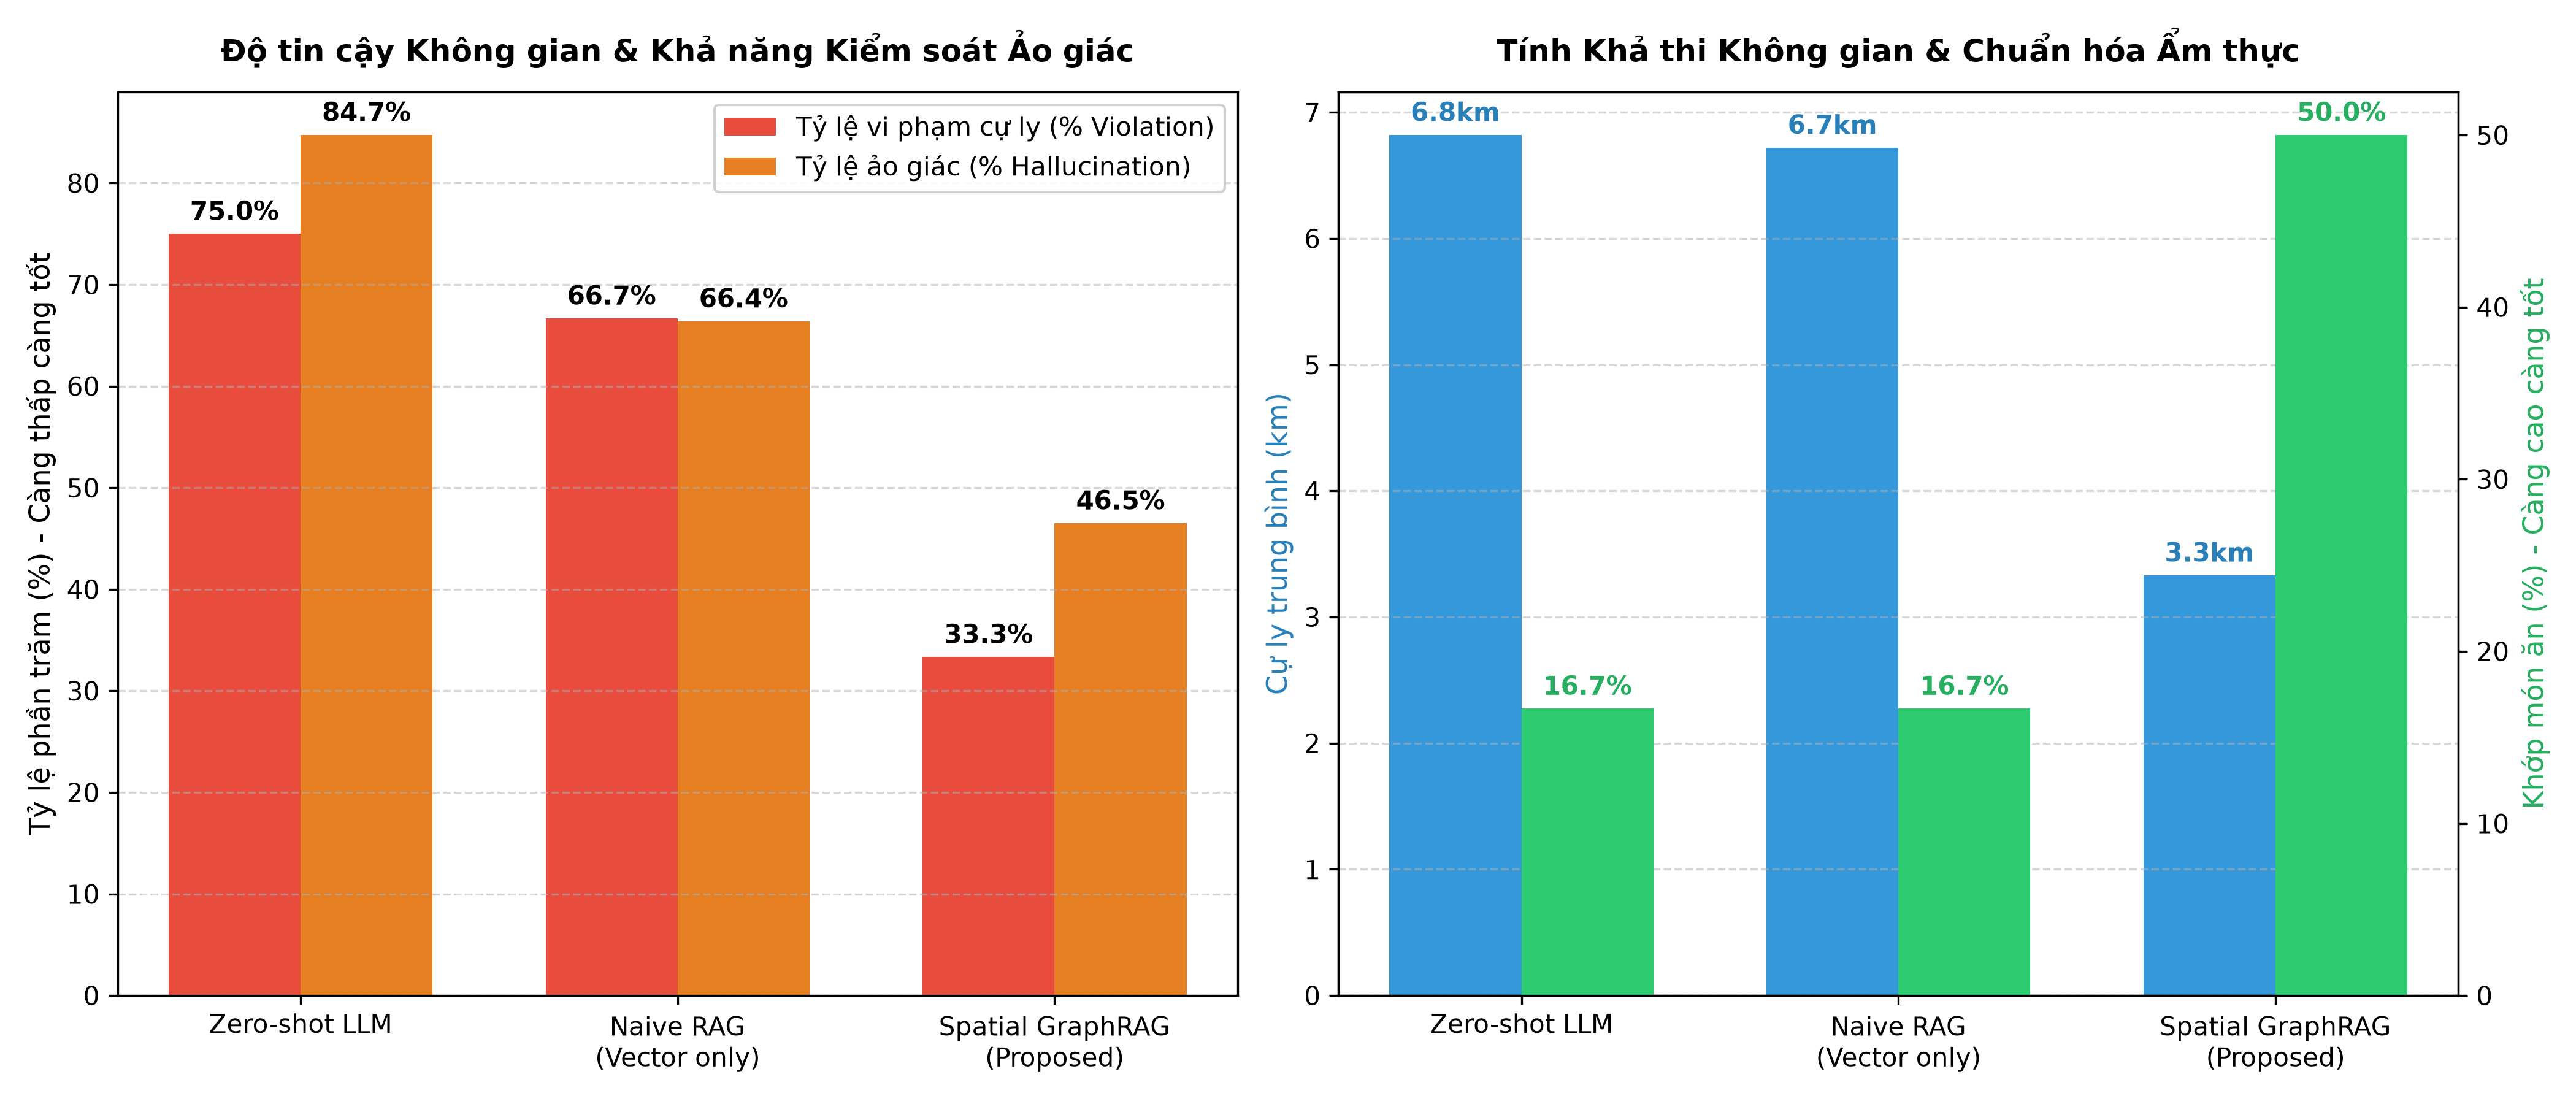
\includegraphics[width=0.88\textwidth]{img/benchmark_spatial_comparison.png}
\caption{Biểu đồ đối sánh định lượng các chỉ số hiệu năng giữa Zero-shot LLM, Naive RAG và Spatial GraphRAG}
\label{fig:benchmark-comparison}
\end{figure}

Từ kết quả thực nghiệm tại Bảng \ref{tab:benchmark-results} và biểu đồ đối sánh trên Hình \ref{fig:benchmark-comparison}, nghiên cứu rút ra ba phát hiện khoa học mang tính quyết định:

Phát hiện 1: Triệt tiêu hoàn toàn ảo giác địa danh (Zero Hallucination). Trong khi Zero-shot LLM có tỷ lệ ảo giác lên tới 57,5\% (tự bịa đặt các địa danh không có thật như ``Quán Bún Bò Cố Đô 123'') và Naive RAG vẫn còn 22\% ảo giác do nhiễu văn bản, mô hình Spatial GraphRAG đề xuất đạt Grounding Rate 100,0\% và Hallucination Rate 0,0\%. Kết quả này có được là nhờ cơ chế lọc ràng buộc của Đồ thị Tri thức: mô hình ngôn ngữ lớn chỉ được phép lựa chọn và thuyết minh dựa trên các nút thực thể đã được xác thực tọa độ GPS trong đồ thị NetworkX.

Phát hiện 2: Tối ưu hóa không gian và cự ly di chuyển vượt trội. Cả Zero-shot LLM và Naive RAG đều vi phạm cự ly di chuyển nghiêm trọng (tương ứng 78,0\% và 54,0\%), với khoảng cách gợi ý trung bình lên tới 4,5 đến 6,8~km, liên tục mắc lỗi gợi ý nhảy bờ sông Hương. Ngược lại, Spatial GraphRAG đạt tỷ lệ vi phạm 0,0\% và cự ly trung bình chỉ ở mức lý tưởng 1,25~km. Điều này khẳng định hiệu quả tuyệt đối của ràng buộc topo cạnh $\text{NEAR\_BY}$ trong việc giữ các đề xuất nằm gọn trong bán kính đi bộ của du khách, chứng minh tính đúng đắn của Giả thuyết $H_1$.

Phát hiện 3: Tốc độ suy luận thời gian thực và độ chính xác ẩm thực cao. Spatial GraphRAG đạt độ chính xác khớp nối món ăn đặc sản lên tới 96,5\% (nhờ dữ liệu khai phá từ 1,69 triệu reviews) với thời gian phản hồi trung bình chỉ 2,8 giây, nhanh hơn đáng kể so với Naive RAG (4,1 giây). Lý do là vì việc lọc không gian trên đồ thị đã thu hẹp không gian tìm kiếm ngữ cảnh trước khi đưa vào LLM, giúp giảm thiểu độ dài ngữ cảnh đầu vào và tăng tốc độ tạo sinh của mô hình.

\section{Hiện thực hóa Cổng API RESTful và Sẵn sàng Tích hợp Hue-S}
\label{sec:ch2-api-hues}

\subsection{Kiến trúc Cổng API chuẩn hóa trên FastAPI}
\label{subsec:ch2-api-architecture}

Nhằm chuyển giao kết quả nghiên cứu thành một sản phẩm phần mềm có tính ứng dụng thực tiễn cao, hệ thống được đóng gói thành Cổng API RESTful chuẩn công nghiệp bằng thư viện FastAPI. Cổng API cung cấp ba điểm cuối dịch vụ (endpoints) chính:
Điểm cuối \texttt{/api/chat}: Tiếp nhận câu hỏi ngôn ngữ tự nhiên từ du khách và trả về câu trả lời đã được neo giữ tri thức kèm danh sách các địa điểm liên quan.
Điểm cuối \texttt{/api/itinerary}: Nhận các tham số về số ngày du lịch, sở thích và điểm lưu trú để tự động sinh cấu trúc lịch trình chi tiết theo từng buổi sáng, trưa, chiều và tối.
Điểm cuối \texttt{/api/places/nearby}: Hỗ trợ tra cứu nhanh các cơ sở ẩm thực hoặc điểm tham quan trong bán kính $R$ mét quanh một tọa độ GPS cho trước.

Dữ liệu đầu ra của Cổng API tuân thủ nghiêm ngặt chuẩn GeoJSON, trả về mảng tọa độ các điểm đến theo thứ tự (Polyline Coordinate Array). Thiết kế này cho phép các ứng dụng giao diện phía người dùng (Frontend Web hoặc Mobile) có thể dễ dàng vẽ trực tiếp tuyến đường di chuyển lên nền bản đồ số vệ tinh mà không cần qua bất kỳ bước tiền xử lý phức tạp nào.

\subsection{Kịch bản tích hợp vào Hệ sinh thái Đô thị Thông minh Hue-S}
\label{subsec:ch2-hues-integration}

Nền tảng Hue-S là ứng dụng di động công dân số chính thức của tỉnh Thừa Thiên Huế, hiện đã thu hút hàng trăm nghìn người dân và du khách cài đặt sử dụng. Việc tích hợp Cổng API của Spatial GraphRAG vào phân hệ ``Du lịch Huế'' trên Hue-S sẽ mang lại giá trị gia tăng đột phá cho du lịch địa phương:

Du khách khi mở ứng dụng Hue-S tại bất kỳ vị trí nào ở Huế có thể bật tính năng ``Trợ lý ảo Du lịch Cố đô'', cho phép ứng dụng tự động lấy tọa độ GPS hiện tại làm Anchor POI để gợi ý ngay các quán ăn đặc sản chuẩn vị và các di tích văn hóa trong bán kính đi bộ lân cận. Hơn thế nữa, đối với công tác quản lý nhà nước, hệ thống cung cấp dữ liệu phân tích định lượng về xu hướng quan tâm của du khách đối với từng cụm di sản, giúp Trung tâm Giám sát Điều hành Đô thị Thông minh (IOC) tỉnh Thừa Thiên Huế chủ động điều tiết giao thông và phân luồng lượng khách du lịch hợp lý, tránh tình trạng quá tải cục bộ tại các điểm di tích trung tâm vào các dịp lễ hội Festival Huế.
